\documentclass[12pt,letterpaper]{article}

\usepackage[utf8]{inputenc}
\usepackage[T1]{fontenc}
\usepackage{amsmath}
\usepackage{amsfonts}
\usepackage{amssymb}
\usepackage{amsthm}
\usepackage[left=2cm,right=2cm,top=2cm,bottom=2cm,headheight=22pt]{geometry}
\usepackage{fancyhdr}
\usepackage{setspace}
\usepackage{lastpage}
\usepackage{graphicx}
\usepackage{caption}
\usepackage{subcaption}
\usepackage{paralist}
\usepackage{url}

\theoremstyle{definition}
\newtheorem{question}{Question}
\newtheorem{example}{Example}
\newtheorem{exercise}[question]{Exercise}
\newtheorem*{challenge}{Challenge}
\newtheorem{theorem}{Theorem}
\newtheorem*{definition}{Definition}
\newtheorem*{lemma}{Lemma}

\begin{document}

%Paramètres de mise en forme des paragraphes selon les normes françaises
\setlength{\parskip}{1ex plus 0.5ex minus 0.2ex}
\setlength{\parindent}{0pt}

%Paramètres relatifs aux en-têtes et pieds de page.
\pagestyle{fancy}
\lhead{Theron J Hitchman}
\chead{\Large Reading and Guided Practice \#04}
\rhead{Spring 2016}
\lfoot{\emph{Math and Decision Making }}
\cfoot{}
\rfoot{\emph{\thepage\ of \pageref{LastPage}}}

\section*{Introduction}

Now we finally reveal the solution to our puzzles: both the Five Cities Puzzle and the Three Utilities Puzzle are 
\emph{impossible}. This the place where I should apologize, but I won't. Instead, I will show you how we use
the ideas we have developed to be \emph{certain} that no one can ever solve those puzzles. This kind of certainty
depends upon the mathematical idea of a \emph{proof}.

\section*{Goals}
At the end of this assignment, a student should be able to:
\begin{compactitem}
\item Say why the graph $K_5$ is not planar.
\item Say why the graph $K_{3,3}$ is not planar.
\item State and use Kuratowski's Theorem describing which graphs are planar.
\end{compactitem}
A student might also be able to:
\begin{compactitem}
\item Discuss what a proof is, and how it is different from other forms of argument.
\end{compactitem}

\section*{Reading and Questions for Graphs Day 4}


So, I have let out the secret. It is impossible to find a solution to either of our two motivating puzzles. 
To understand why, we will explore several \emph{proofs}. For context, we will discuss the idea of a proof, and 
why it is a special thing. And then we will learn a neat theorem that handles the whole question of ``Which graphs
are planar?''


\subsection*{The Idea of a Proof and a Key ``Lemma''}

What is a \emph{proof}? The simplest explanation is that it is a convincing argument. But there is more to it 
than that: human beings make convincing arguments all the time without getting all the way to a ``proof.'' 
In particular, many parts of human experience and thought are just fine with something more like ``a statistical 
preponderance of evidence.'' A person gathers so much information, so many examples, so much related data that 
they eventually things can't reasonably be otherwise and they decide that is enough to be convincing. All of the doubts the person has are so small and so unlikely that he or she just decides to get on with life.

But mathematicians are the most skeptical lot of people you can imagine. When we demand a proof, we mean an 
argument that removes \textbf{all} doubts. By all doubts, I mean not only those you can imagine right now, but any
and all \emph{future} doubts, too. A proof is an argument that covers every single case. All of them.

Naturally, coming up with mathematical proofs is really hard work. This is the reason that mathematicians demand
very precise use of language ---  writing a proof is generally impossible without precise terms. But the other 
side of this coin is that mathematicians only try to talk about special types of things: numbers and shapes. No
mathematician will attempt to prove a theorem about the behavior of toddlers, for instance.


Oh, I just used another special word. A \emph{theorem} is a mathematical statement which has been deemed true
because it has an accepted proof. There are lots of words mathematicians use as synonyms for theorem. We'll need 
one now. A \emph{lemma} is a little helper theorem that might not be so interesting on its own, but does a lot of 
work to help us structure proofs of other theorems which are considered more important.

For example, here is a lemma about graphs with planar drawings that will be very helpful.

\begin{lemma}[Planar Drawing Cycles Lemma]
Suppose that a graph $G$ has a simple cycle in it. Then in any planar drawing of $G$, we cannot have a pair of
vertices $v_1$ and $v_2$ such that 
\begin{itemize}
\item $v_1$ lies inside the cycle,
\item $v_2$ lies outside the cycle, and 
\item $v_1$ and $v_2$ are joined by an edge.
\end{itemize}
\end{lemma}

\begin{proof}[Proof of the Planar Drawing Cycles Lemma]
Suppose that we have a planar drawing of a graph $G$ which has a cycle in it. This cycle will divide the plane into two regions, an inside and an outside.  

If we were to draw a vertex $v_1$ which lies on the inside and a vertex $v_2$ which lies on the outside, then 
\textbf{any} edge joining $v_1$ to $v_2$ has to cross the cycle at some point. 

But if that happens, the drawing is not a planar drawing. So, we cannot have such a pair of vertices.
\end{proof}

\begin{exercise}
Draw a cycle out of a chain of vertices and edges. Then draw a vertex $v_1$ inside the cycle and a vertex $v_2$ outside the cycle.  See that there is no place to put the edge between $v_1$ and $v_2$. Just try it.
\end{exercise}

\begin{exercise}
Recall that we have already learned a theorem, and we discussed a proof of it in class. What was that theorem?

Do you recall how the proof goes?
\end{exercise}


Now we turn to proving the main results of the day. If all goes well, you will understand two proofs for each theorem. That makes us double-sure. (smiley face goes here)

\clearpage

\subsection*{First Method and the Non-Planarity of $K_5$}

Now it is time for a big theorem. This proves that the Five Cities puzzle is impossible to solve.

\begin{theorem}\label{thm:k5}
The graph $K_5$ has no planar drawing.
\end{theorem}

\begin{exercise}[To be done during your reading of the proof!]
Draw your own figures as you read the proof below. This is the best way to understand the argument.
In fact, it is so important that I will not draw the figures for you. Draw for yourself!
\end{exercise}

\begin{proof}
Note that since $K_5$ is the complete graph on five vertices, every set of three vertices is part of a 3-cycle --- a triangle!

Label the vertices of $K_5$ with the letters $A, B, C, D$, and $E$.

Suppose that we can make a planar drawing of $K_5$. Then we must be able to draw the 3-cycle with vertices $A, B$, and $C$.  We will consider all of the possible cases for where we can place the other two vertices $D$ and $E$, and show that none of them can work. A key tool will be the Planar Drawing Cycles Lemma.

Here is a list of all the possible ways we can place $D$ and $E$.
\begin{enumerate}
\item $D$ lies inside the triangle $ABC$ and $E$ lies outside the triangle $ABC$,
\item $E$ lies inside the triangle $ABC$ and $D$ lies outside the triangle $ABC$,
\item both $D$ and $E$ lie inside the triangle $ABC$, 
\item both $D$ and $E$ lie outside the triangle $ABC$.
\end{enumerate}

Our first observation is that cases (1) and (2) are impossible by the Planar Drawing Cycles Lemma. In both, the vertices $D$ and $E$ are on separated by the triangle, so we cannot draw the edge $DE$ without making a crossing.
So we conclude that cases (1) and (2) cannot happen.

Now suppose that we are in case (3), where both $D$ and $E$ lie inside the triangle. First draw $D$, and then draw 
edges $DA$, $DB$ and $DC$. This divides the interior of the triangle $ABC$ into three parts. We must have that $E$
lies inside one of them. Each of these three cases is completely similar, so we will just assume that $E$ lies inside
the triangle $ABD$. 

So, we are in the case where $E$ lies inside the 3-cycle $ABD$, but $C$ lies outside that 3-cycle. So by the Planar
Drawing Cycles Lemma, it is impossible to draw the edge $CE$ without making a crossing. We conclude that case (3)
cannot happen.

Finally, consider case (4), where $D$ and $E$ lie outside the triangle. Again, place $D$ somewhere outside the
3-cycle $ABC$. Then draw edges $DA$ and  $DB$ which do not cross any other part of the figure. This divides 
the region outside of the 3-cycle $ABC$ into three parts: inside the 3-cycle $BCD$, inside the 3-cycle $ACD$ and outside the 3-cycle $ABD$. We must place $E$ into one of these three.

In each case, we end up in the situation of the Planar Drawing Cycles Lemma: there will be a 3-cycle which separates
a pair of vertices. In this set up, $E$ will always be one of the vertices which causes trouble. We conclude that case (4) is impossible.

Well, that is it. We have seen that there are only four possible cases. But each of these four cases is impossible.
Therefore, it is impossible to find a planar drawing of $K_5$.
\end{proof}


Wasn't that satisfying? If you have to, go back and read it again. Draw the pictures anew. 

That probably felt long to you. But notice there is really only one key idea: $K_5$ has a lot of three cycles in it, and that means we can use the Planar Drawing Cycles Lemma a lot.


\begin{exercise}
Go back to our first reading and refresh your memory of the idea of the \emph{crossing number} of a graph.
\end{exercise}

\begin{exercise}
Give a proof for why the crossing number of $K_5$ is $\mathrm{cr}(K_5) = 1$.
\end{exercise}


\begin{challenge}
Consider the graph $K_{3,3}$. Instead of triangles, the simplest cycles in this graph are all squares, that is, 4-cycles.
Can you use the method of the proof above to argue that $K_{3,3}$ has no planar drawing?
\end{challenge}


\clearpage

\subsection*{Second Method and the Non-Planarity of $K_{3,3}$.}


Now, let's look at the graph from the Three Cities Puzzle. We will use a different method to show that it has no planar drawing. This time, we will rely on Euler's Formula.

\begin{theorem}\label{thm:k33}
The graph $K_{3,3}$ has no planar drawing.
\end{theorem}

\begin{exercise}
Draw pictures and work the details of this proof for yourself as you read. 
If there is a step you don't understand, make a note of it by writing down a careful question.
Later, you should talk to someone about your question.
\end{exercise}

\begin{proof}
Suppose that it were possible to make a planar drawing of $K_{3,3}$. The smallest simple cycles in this graph
are 4-cycles, that is, squares. Because of the Planar Drawing Cycle Lemma, each such simple cycle has to contain either all of the other vertices of the graph, or none of them. This means we can count the regions in Euler's formula by counting the simple 4-cycles. A careful count shows that $K_{3,3}$ has $9$ different 4-cycles. Each one is a square made of two vertices from each of the subsets.

So now we count. The graph has $V=6$ vertices, and $E = 9$ edges. By Euler's Formula, we know that
\[
2 = V- E + R = 6 - 9 + R.
\]
This means that $R$ must be equal to $5$. That is we must have $5$ regions in a planar drawing of $K_{3,3}$.

But we have already seen that there must be one region for each 4-cycle, and there are $9$ of those! This mismatch
means that it is impossible to make a planar drawing of $K_{3,3}$.
\end{proof}

\begin{exercise}
Give a proof for why the crossing number of $K_{3,3}$ is $\mathrm{cr}(K_{3,3}) = 1$.
\end{exercise}


\begin{challenge}
Consider the graph $K_5$.  Can you use the method of the proof above to argue that $K_5$ has no planar drawing?
This would mean that you have \emph{two} proofs of Theorem \ref{thm:k5}.
\end{challenge}

All the same, if you complete the challenge in the last section, you have two proofs of Theorem \ref{thm:k33}.

\clearpage

\subsection*{Kuratowski's Theorem and the Complete Understanding of Planarity}

Now, to finish up, there is a theorem that gives us a way to test if any graph has a planar drawing or not. It depends on the idea of a \emph{subdivision} of a graph.

Let $G$ be a graph. A \emph{subdivision} of $G$ is a graph which is obtained by splitting an edge of $G$ into two edges by putting a vertex somewhere in the middle of that edge, and possibly doing this a large number of times.

For example, here is the complete graph on 3 vertices, $K_3$, and a subdivision of it.

\begin{figure}[h]
\centering
\begin{subfigure}[b]{.4\textwidth}
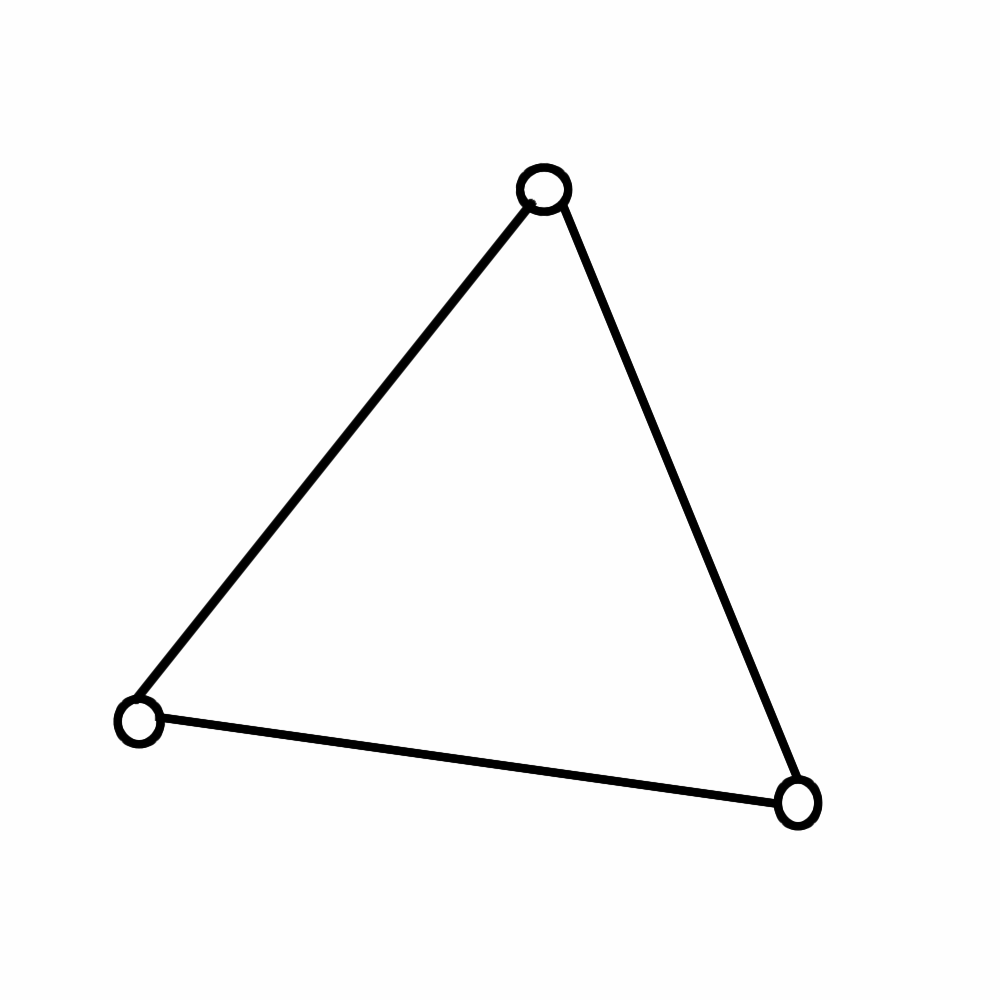
\includegraphics[width=\textwidth]{images/k3.png}
\caption{The graph $K_3$}
\end{subfigure}
\begin{subfigure}[b]{.4\textwidth}
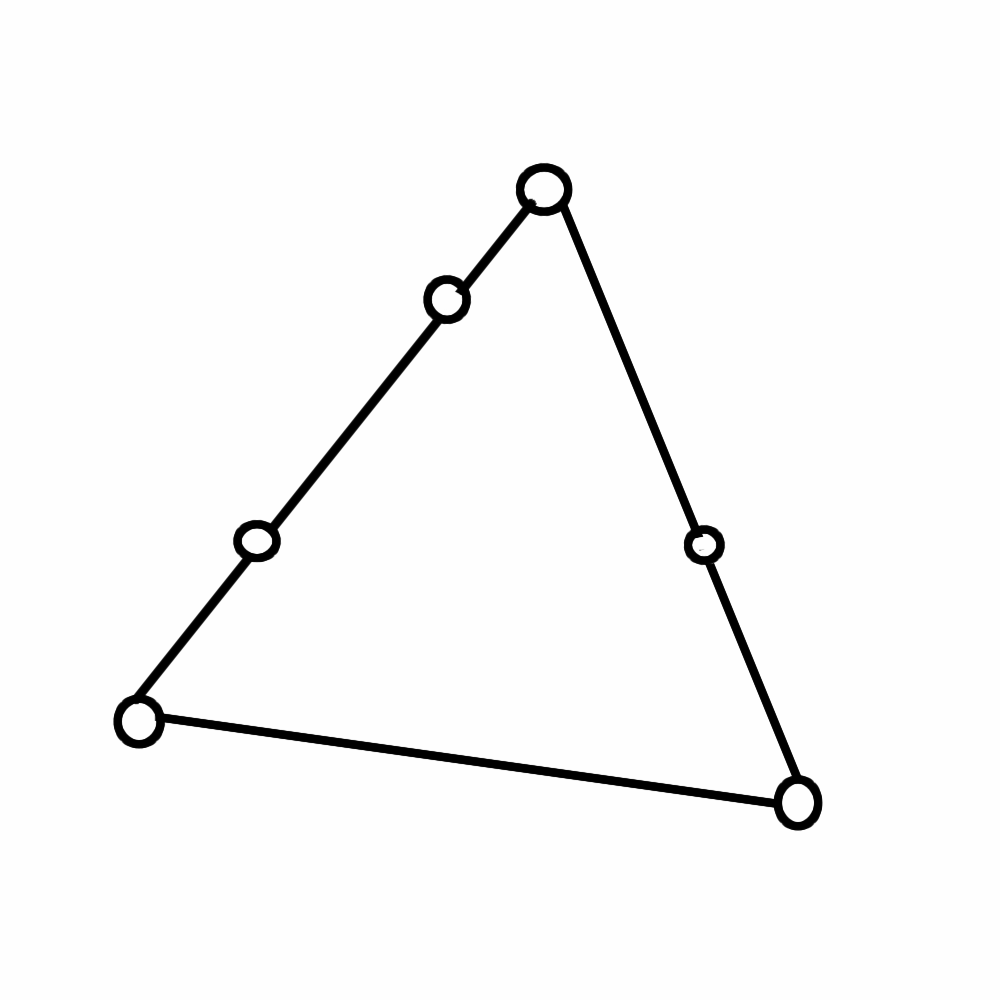
\includegraphics[width=\textwidth]{images/k3subdiv.png}
\caption{A subdivision of $K_3$}
\end{subfigure}
\caption{An example of subdivision}
\end{figure}


\begin{exercise}
Draw a few different graphs which are subdivisions of $K_{3,3}$.
\end{exercise}


\begin{theorem}[Kuratowski's Theorem, \cite{kuratowski}]
A graph fails to be planar exactly when it has either 
\begin{itemize}
\item a subgraph which is a subdivision of $K_5$, or
\item a subgraph which is a subdivision of $K_{3,3}$.
\end{itemize}
\end{theorem}


\begin{exercise}
Design a graph which you know has to be planar.
\end{exercise}

\begin{exercise}
Design a new graph which you know for sure is \textbf{not} planar.
\end{exercise}

\begin{thebibliography}{9}

\bibitem{kuratowski}
  Casimir Kuratowski,
  ``Sur le {probl\`{e}me} de courbes gauche en Topologie,''
  \emph{Fund. Math.} \textbf{15}: 271-283.
  available at: \url{http://matwbn.icm.edu.pl/ksiazki/fm/fm15/fm15126.pdf}
  (in French)

\end{thebibliography}

\end{document}
%sagemathcloud={"zoom_width":100}












